
% \addtocontents{toc}{\protect\vspace{\beforebibskip}}%
%\chapter*{Mapping Animal Movement in \textit{R}: The Science and the Art}
%\chaptermark{Mapping Animal Movement in \textit{R}: The Science and the Art}
\phantomsection
\begin{addmargin}[-3cm]{-1.5cm}
	
	\fcolorbox{Black}{Snow2}{
		\begin{minipage}[t]{\linewidth}%{\dimexpr\linewidth-2\fboxsep}
			%\phantomsection
			% \addtocontents{toc}{\protect\vspace{\beforebibskip}}%
			\addcontentsline{toc}{chapter}{\tocEntry{\color{gray}\bfseries{Mapping Animal Movement in \textit{R}}}}%
			{\small \color{SteelBlue4} \chapter*{Mapping Animal Movement in \textit{R}} }
			\chaptermark{}
			
			\centering
				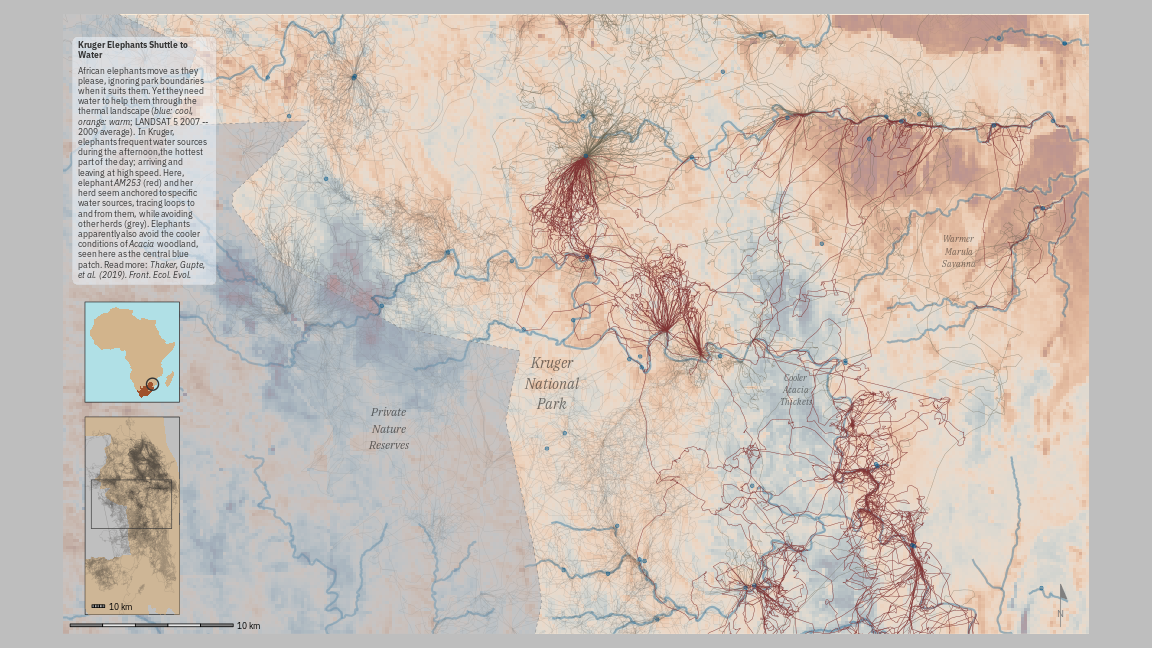
\includegraphics[width=15cm]{figures/boxes/elemove.png}
			\label{fig:sample_figure}
			
			
		
		\end{minipage}
	}
	
\end{addmargin}

% \begin{tcolorbox}[
%   blanker,
%   width=0.99\textwidth,
%   before skip=6pt,
%   colback=gray,
%   breakable]

% {
%     \pdfbookmark[1]{Mapping Animal Movements: The Science and the Art}{Mapping Animal Movements: The Science and the Art}
%     \addcontentsline{toc}{chapter}{\color{gray}\tocEntry{Mapping Animal Movements: The Science and the Art}}

%     {\sffamily{Pratik R. Gupte}}

%     \footnotesize\sffamily

%     In December 2020 I was pointed to the BES Mapping Animal Movements Contest, and the “R Map” category stood out to me. I entered a map made showing the movement of 14 savanna elephants Loxodonta africana tagged in Kruger National Park, South Africa.

%     The map highlights the path of the female elephant AM253 (the tag number). Some of the thirteen other elephants are also shown to give a sense of how densely Kruger is criss-crossed by elephant herds. The background shows the average temperature sensed by the LANDSAT-5 satellite over the two year period of this study.

%     This data was part of the postdocs of Maria Thaker and Abi Vanak, for whom I worked between my master’s and my PhD. We wrote a paper about how Kruger elephants move in response to temperature. The source code and the map I made can be found here.

%     \section{Mapping as Exploratory Data Analysis}

%     Mapping animal movements is a key component of exploratory data analysis. It’s important for ‘joining the dots’ of animal positions. Large tracking datasets can contain errors that are only evident to researchers when they look at an approximation of the animal’s path and ask, “Does the animal move this way?”

%     For instance, this map shows ‘jumps’: long, linear segments between points, which indicate missing data for some periods. Mapping can also reveal interesting behaviours that can only be observed after significant effort in the field.

%     For instance, the ‘looping’ behaviour of AM253 to water sources is the focus of this map. Seeing this looping behaviour allowed us to focus our study on elephant movements between visits to water sources.

%     \section{Mapping as Art}
    
%     As with many other areas of science (other than primary data collection, please!), when in doubt about maps, copy.

%     Growing up in early 2000s India, I read hard copies of National Geographic Magazine, which has long had fantastic graphics. Where the Animals Go was a source of inspiration as well. I picked up other tips and tricks from knowing something of art generally: build up an image in layers, use colours that don’t clash, highlight the phenomenon of interest. Interestingly, some of these approaches are very much in line with the ‘grammar of graphics’ approach of ggplot, which I used to make this map.

%     \section{Mapping in R}

%     Getting Temperature Data or A Detour with Python

%     I used LANDSAT-5 for the temperature layer because it was the appropriate satellite for the time period (2007), and had a decent spatial resolution (30 metres). I used Google Earth Engine (GEE) to acquire this data. The heavy computation happens on the GEE servers, significantly increasing speed. By collecting these data for use at one point, GEE also improves data accessibility.

%     I used Python to get the LANDSAT-5 data from Google Earth Engine, using the ee package, which is the Python GEE API package. The rgee R package is similar, but works via Python, so I used Python directly.

%     I found Qiusheng Wu’s geemap package a great tool for visualisation of the data I was working with, and the associated tutorials a very good resource for help with ee generally.

%     \section{Getting Elephants and Other Landscape Features}

%     In 2019, we published the data on the Movebank data repository (It now forms part of the animation on the starting page). Getting the data was thus very easy using the move package, which I then saved as a geopackage.

%     I acquried the river course data using the osmdata package, which queries and retrieves data from the OpenStreetMap database. The boundaries of Africa and South Africa come from the rnaturalearth package. The Kruger boundary and the locations of waterholes originally come from the South African National Park service.

%     \section{Choosing Mapping Tools}

%     R’s great advantage over other languages is visualisaton, specifically the popular ggplot package. ggplot’s emergence as a mainstay of spatial visualisation is due to its geom\_sf function, which can handle sf spatial objects.
    
%     One of ggplot’s advantage’s is its many extensions. Here, I used the ggspatial and ggtext extension packages to add the scale bars and north arrow, and to add the text box, respectively.
    
%     Plotting rasters is not straightforward in ggplot. There are two main options: the stars package and its associated geom\_stars, or converting a raster dataset into a dataframe with regular coordinate intervals and using geom\_tile.
    
%     Here, I chose the second approach because I’m an infrequent stars user; since making the map I’ve tried geom\_stars which works just as well, and is very convenient.

%     \section{Choosing Map Colours}

%     I coloured the temperature raster using the scico package’s ‘VikO’ palette. I tried out a number of palettes from the scico, pals (providing the Kovesi palettes), RColorBrewer, and colorspace packages. I chose a diverging palette to show heterogeneity in the thermal landscape, but this approach is not to be recommended for material that will be printed in grayscale.

%     \section{Reproducibility in R}

%     I adopted a relatively relaxed understanding of reproducibility: given the data, the code would be reproducible if it could produce the map I had entered for this contest. To do this, I set up a continuous integration pipeline using Github Actions (GHA).

%     Using the usethis package, I created a DESCRIPTION file, which is usually reserved for packages. This file tricks GHA into reading its contents, especially the dependencies, i.e., the R packages required by the project.

%     GHA automatically reads the dependencies and installs them, as well as the programs required by those dependencies. For instance, GDAL (the Geospatial Data Abstraction Library) is key to nearly all spatial analyses, and is installed as a requirement of the rgdal package, which is itself key to sf and raster.

%     I used the R package renv to make sure that the packages (and the package versions) I used are available to the pipeline. renv creates a lockfile, a registry of packages the current project uses, from which those packages can be installed.

%     Finally, to check whether the entire pipeline works, I used bookdown to sequentially execute the series of Rmarkdown files. An obvious alternative is rmarkdown.

%     GHA runs this pipeline and reports whether the code ran successfully, and if not, where it failed (you can see these reports here). GHA runs the pipeline on Linux, and Windows containers (Mac OS-x is also supported). This means that though I use Linux, I’m pretty sure that this code works for Windows users.

%     \section{The Limits of Reproducibility}

%     Reproducibility inevitably breaks down at certain scales in an ecological study. For instance, it would be impossible to reproduce the primary data collection of the study, such as which elephants were captured and fitted with transmitters. These data are taken on faith from the original researchers, highlighting the role of trust in the scientific community.

%     Code too is not exempt from reproducibility limits. For instance, restoring the renv lockfile is very difficult without an internet connection, as packages may need to be downloaded.

%     In ten years, code in R or another language may no longer be reproducible due to software and hardware changes, as many researchers found in the 10-year reproducibility challenge. Finally, entire services might become unavailable; for example, the raster processing using Google Earth Engine is dependent on Google maintaining this service.

%     Researchers then, should be pragmatic about reproducibility. Who is it for — the researchers themselves, the reviewers of their manuscript, their students, their funders?

%     To whom is this effort owed, and by whom, and how can the additional work required be prevented from becoming a gatekeeping mechanism (1), (2)? These are issues that the ecology and evolution community will have to address.
% }

% \end{tcolorbox}
